\chapter{Структура системы передачи информации}

Система передачи информации показана на Рис.~\ref{img_01}. Она состоит из источника информации, генерирующего исходный 
поток данных. Источник информации передает данные в кодер источника информации, который предназначен для устранения 
естественной избыточности генерируемой информации. Кодированные данные затем поступают в кодер канала. Данный 
компонент предназначен для кодирования данных помехоустойчивым кодом для возможности обнаружения ошибок на удаленной 
стороне и восстановления исходных данных.

\begin{figure}[htbp]
\begin{center}
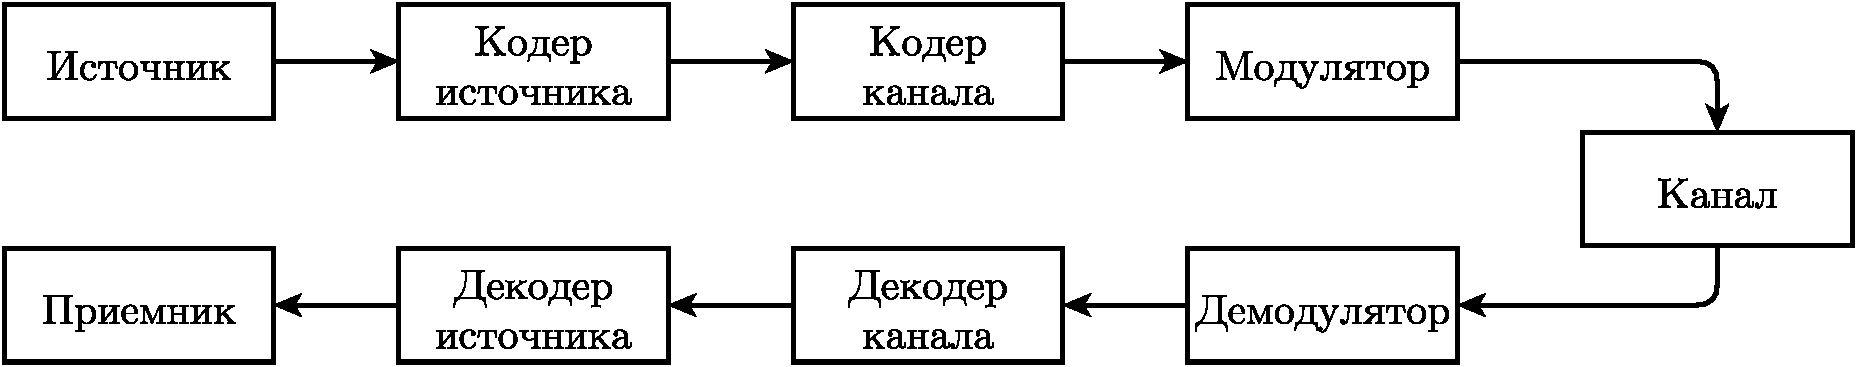
\includegraphics[scale=0.45]{chapter_1/img_01.pdf}
\end{center}
\caption{Структура системы передачи информации}
\label{img_01}
\end{figure}

Таким образом, кодированные данные поступают в модулятор, который предназначен для генерации по цифровым данным реальных физических сигналов и их передачу в канал. Причем в данной ситуации каналом может являться как телефонный кабель, оптическое волокно, воздушная среда, так и система хранения информации, например, жесткий диск, магнитный диск или флеш- накопитель. По сути, все эти устройства реализуют канал связи, который в общих чертах можно охарактеризовать как компонент, позволяющий передавать данные и обладающий тем свойством, что при передаче данных могут возникать ошибки. Их появление объясняется природой канала и не может быть определено заранее. После передачи данных каналом и получения данных на удаленной стороне начинается обратный процесс, нацеленный на восстановление переданных данных. Вначале данные из канала демодулируются демодулятором, который генерирует кодовые слова выбранного кода. Данные слова декодируются декодером канала. В случае обнаружения декодером ошибок при передаче данных, выполняется процесс устранения данных ошибок с целью получить исходные денные. В результате декодирования данные поступают в декодер источника. На этом этапе выполняется декодирование данных, изначально сгенерированных источником, добавляется избыточная информация. Полученные денные отправляются приемнику информации.